\chapter{MULTI-PORT RAM}
\label{chapter:scratchpad}
\section{Introduction}
Our multi-port RAM was created to allow mutliple processing elements to use a shared memory. It is a component in the larger design for a sparse matrix vector multiplier. Specifically it allows the decoder to access more memory space without going off chip. The component allows each PE to access a table that is 16 times larger than if it was stored inside each PE. Multi-port RAMs have been designed before, but none achieve our desired performance.


Following Moore's Law, transistor densities on FPGAs continue to increase at an exponential rate~\cite{fpga_2032}. This allows for increasingly complex System-on-Chip implementations that require high throughput communication and shared memory on networks of distributed compute nodes. ASIC designs used as accelerators in the field of high-performance computing often utilize multi-port memories for communication. By comparison, FPGA vendors do not provide scalable multi-port memories in their fabric, with most device families being limited to using dual-port memories~\cite{f-scratch:altera, f-scratch:xilinx}. In these cases designers must use a multi-port memory constructed with FPGA logic and RAM blocks. These soft IP cores consume significant resources if the memory must behave identically (in terms of performance) as an ASIC equivalent. As an alternative design strategy, if the multi-port memory can stall and exhibit variable multi-cycle latencies, substantially fewer resources can be used. Heavily pipelined processing elements can often tolerate these restrictions.

In this paper we present two FPGA-based multi-port memory designs that allow for scalability in terms of the number of ports as well the addressable memory space. By providing a banked RAM block architecture, our designs allow for implementations that support up to 256 ports and 1MB of memory space on current-generation FPGA devices. In contrast to previous banked implementations in the research literature, our multi-port memories utilize buffering and reordering of memory requests. This results in throughput that approaches the ideal-case throughput, while providing an unsegmented address space. An unsegmented address space allows for simpler integration with the rest of an accelerator implementation.

The rest of this paper is organized as follows. Section~\ref{sec:relatedwork} provides an overview of related work in multi-port memory design. In Section~\ref{sec:architecture}, we present our two designs (the Fully-connected and Omega memories), which provide for an explicit trade-off between implementation complexity and achievable throughput. A discussion of our evaluation methodology is provided in Section~\ref{sec:evaluation} followed by an analysis of resource usage and performance in Section~\ref{sec:analysis}. Finally, the paper is concluded with a detailed view towards planned future work in Section~\ref{sec:conclusion}. 


\section{Related Work}
\label{sec:relatedwork}

If a multi-port memory only requires a small amount of memory space, one can synthesize the multi-port memory using only FPGA logic resources, as seen in \cite{f-scratch:jones}. Otherwise, soft multi-port memories utilize the dual-port RAM blocks available on most FPGAs. A review of the research literature illustrates the four design strategies using dual-port RAM blocks: {\em multi-pumping}, {\em replication}, {\em Live Value Table}, and {\em banking}.

{\em Multi-pumping}, seen in \cite{f-scratch:manjikian,f-scratch:canis,f-scratch:yantir}, gains ports by using an internal clock and an external clock, with a clock speed of a constant multiple slower than the internal clock. This way the RAM block can process the requests of multiple ports. This approach limits the number of ports, as each added port decreases the maximum clock frequency.

{\em Replication}, seen in \cite{f-scratch:fort,f-scratch:mousali,f-scratch:yiannacouras}, gains read-only ports by connecting the write ports of multiple RAM blocks together. This approach does not sacrifice clock speed or FPGA logic resources. However, each extra RAM block just provides one read-only port. Also, increasing the RAM blocks does not expand the storage space of the memory, since the data is explicitly replicated among the blocks.

{\em Live Value Table}, seen in \cite{f-scratch:laforest,f-scratch:anjam,f-scratch:abdelhadi}, gains ports by using a quadratically growing number of RAM blocks. This approach generates an $N \times N$ array of RAM blocks to create $N$ ports. Similar to replication, Live Value Table connects the write ports of all the RAM blocks in each row. During a write, a port writes to all the RAM blocks in one row. During a read, a port reads from all the RAM blocks in one column. One of the outputs from this column contains the most recent and the correct value for the read response. A ``Live Value Table'' keeps track of this information. Other techniques use an XOR operator instead of a Live Value Table \cite{f-scratch:laforest2}. These approaches have the advantage of low latency and working at relatively high frequencies. A significant drawback is the resource usage, since the number of extra RAM blocks scales quadratically with the intended memory size. Another drawback, which this approach shares with replication, is that these added RAM blocks do not expand the storage space of the memory.

{\em Banking}, seen in \cite{f-scratch:moscola,f-scratch:saghir,f-scratch:saghir2}, gains ports by adding RAM blocks to expand the memory. This allows the memory to gain a full port and increase the memory space. However, multiple ports can not access the same RAM block (and therefore the unique memory space it holds) at the same time. Also, some type of network must route signals between the ports and the banks. These previous banking approaches do not buffer requests and therefore restrict the access of each port to a fraction of the memory space, explicitly segmenting each bank. By comparison, the work presented in this paper buffers and reorders messages, allowing unsegmented access to memory.

\section{Architecture}
\label{sec:architecture}
    \begin{figure}
        \center
        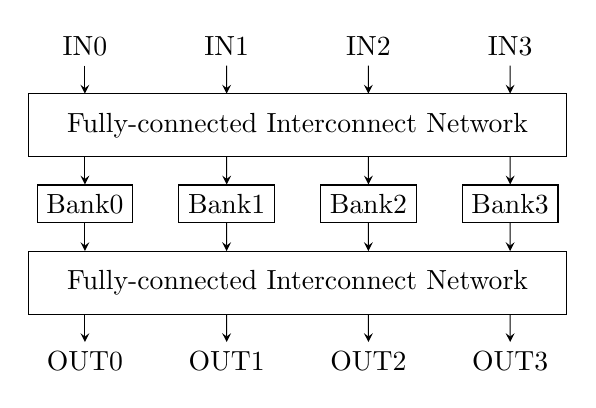
\begin{tikzpicture}[xscale=1.8]
            \draw (-.4,-1.6) rectangle (3.4,-2.4);
            \draw (-.4,-3.6) rectangle (3.4,-4.4);
            %\draw[dashed] (-.5,-1.5) rectangle (3.5,-4.5);
            \foreach \x in {0,1,...,3}{
                \node at (\x,-1)(in){IN\x};
                \node at (\x,-5)(out){OUT\x};
                %\draw[xshift=\x cm - .1 cm,fill=white](-.3,-.6) -- (-.3,-.8) -- (.5,-.8) -- (.5,-4.7) -- (-.3,-4.7) -- (-.3,-5.3) -- (.6,-5.3) -- (.6, -.6) -- cycle;
                %\node at (\x, -5){Reorder};
                \node[draw] at (\x,-3)(mem){Bank\x};
                \path[draw,>=stealth,->] (in) -- (\x,-1.6);
                %\path[draw,>=stealth,->] (\x,-.8) -- (\x,-1.6);
                \path[draw,>=stealth,->] (\x,-2.4) -- (mem);
                \path[draw,>=stealth,->] (mem) -- (\x,-3.6);
                %\path[draw,>=stealth,->] (\x,-4.4) -- (\x,-4.7);
                \path[draw,>=stealth,->] (\x,-4.4) -- (out);
            }
            \node[fill=white] at (1.5,-2){Fully-connected Interconnect Network};
            \node[fill=white] at (1.5,-4){Fully-connected Interconnect Network};
            %\node[xshift=-3,rotate=90,fill=white] at (-.5,-3){Multi-port Memory};

        \end{tikzpicture}
        \caption{In the Fully-connected multi-port memory all the buffering occurs in the fully-connected interconnect networks.}
        \label{fig:fullmemory}
    \end{figure}


As previously mentioned we implemented two different memory designs, hereafter referred to as the {\it Fully-connected} and {\it Omega} multi-port memories. As will be further demonstrated in Section~\ref{sec:analysis}, a key differentiator is that the Fully-connected memory has better throughput, while the Omega memory scales better in terms of resource usage. However, both memories share common characteristics. Both designs use single-port RAM blocks for the memory banks, and utilize reorder queues. Also, both utilize a network structure for routing between ports and banks, and buffer requests to resolve contention. 

\subsection{Fully-connected Multi-port Memory}
    The Fully-connected multi-port memory (\figurename~\ref{fig:fullmemory}) uses fully-connected interconnect networks. The first fully-connected network routes requests from the input ports to the banks. The second routes read responses from the banks to the output ports.
\subsubsection{Memory Banks}
For any banking approach, a memory with $N$ ports requires at least $N$ RAM blocks. Each RAM block holds a unique segment of the total memory space. We have multiple options to decide how to segment the memory space. The simplest option assigns the first $N^{th}$ of the address space to Bank0, the next $N^{th}$ to Bank1, and so on. However, this approach can easily cause bottlenecks. For example, assume all the processing elements start to read from a low address located in Bank0 and continue to sequentially increment the read addresses. All the requests would route to Bank0, necessitating multiple stalls. The interleaving memory address space that our design uses decreases the chance these specific types of bottlenecks occur.
\subsubsection{Fully-connected interconnect network}
    \begin{figure}
        \center
        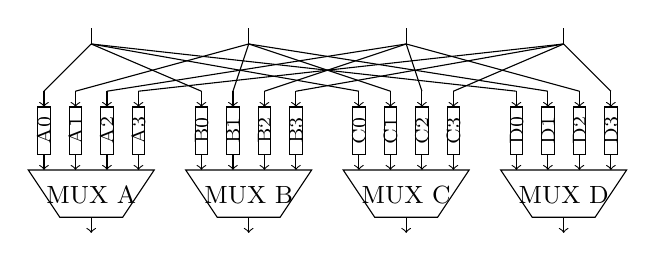
\begin{tikzpicture}[scale=.4]
            \foreach \i/\l in {0/A, 5/B, 10/C, 15/D}{
                \draw[xshift=\i cm] (-2,1) -- (2,1) -- (1,-.5) -- (-1,-.5) -- cycle;
                \node at (\i,.2){\small MUX \l};
                \draw [xshift=\i cm,->](0,-.5) -- (0,-1);
                \foreach \j/\p in {-1.5/0, -.5/1, .5/2,1.5/3}{
                    \draw [xshift = \i cm](\j-.2,1.5) rectangle (\j+.2,3);
                    \node at (\i+\j,2.25)[rotate=90]{\scriptsize \l\p};
                    \draw [xshift = \i cm,->](\j,1.5) -- (\j,1);
                    \draw [xshift = \i cm,->](\j,3.5) -- (\j,3);
                }
            }
            \foreach \i/\j in {0/-1.5, 5/-.5, 10/.5, 15/1.5}{
                \foreach \k in {0, 5, 10, 15}{
                    \draw (\i, 5) -- (\k+\j, 3.5);
                }
                \draw (\i,5) -- (\i, 5.5);
            }
        \end{tikzpicture}
        \caption{Fully-connected interconnect network}
        \label{fig:crossbar}
    \end{figure}

    A fully-connected interconnect network (Fig.~\ref{fig:crossbar}) consists of multiple arbiters. An arbiter routes data from several inputs to one output, and typically consist of simple FIFOs, a multiplexer, and some control logic. In Fig.~\ref{fig:crossbar}, FIFOs A0 to A3 and MUX A construct one of the four arbiters needed for a four-port fully-connected interconnect network.

We use a simple round robin scheme to resolve contention. Assuming the arbiter most recently read from FIFO A0, the arbiter would continue to read from FIFO A0 until it is empty. Then, the arbiter reads from FIFO A1. Again, the arbiter continues to read from FIFO A1 until it is empty, and the cycle repeats. This control scheme has the advantage that it achieves high throughput and requires little control logic.

Generally, a $N$-by-$N$ fully-connected interconnect network consists of $N$, $N$-to-$1$ arbiters. The arbiters act independently. This independence allows for good arbitration schemes that achieve high throughput and low latency.
Unfortunately, as the size of a fully-connected interconnect network grows, the more space the FIFOs and multiplexers require. A 8-to-1 multiplexer requires approximately twice the number of resources of a 4-to-1 multiplexer. This means the area the multiplexers require grows by around $N^2$. The number of FIFOs grows by $N^2$ as well.

%\begin{figure}
%    \center
%    \input{fig/arbiter.tex}
%    \caption{Arbiter}
%    \label{fig:arbiter}
%\end{figure}


\subsection{Omega Multi-port Memory}
    \begin{figure}
        \center
        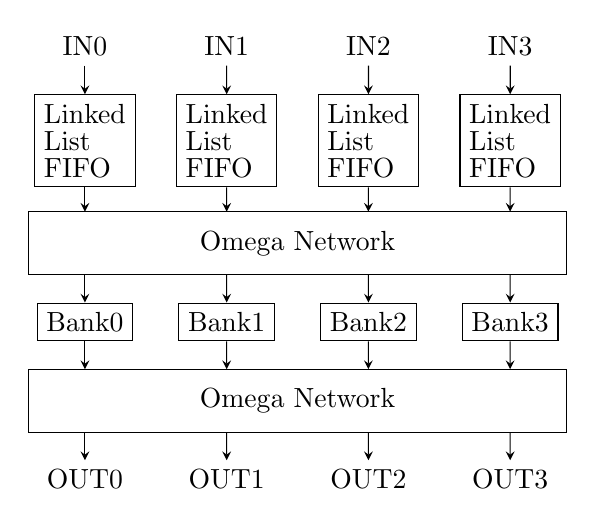
\begin{tikzpicture}[xscale=1.8]
            \draw (-.4,-1.6) rectangle (3.4,-2.4);
            \draw (-.4,-3.6) rectangle (3.4,-4.4);
            %\draw[dashed] (-.5,0) rectangle (3.5,-4.5);
            \foreach \x in {0,1,...,3}{
                \node at (\x,.5)(in){IN\x};
                \node at (\x,-5)(out){OUT\x};
                %\draw[xshift=\x cm - .1 cm,fill=white](-.3,.5) -- (-.3,.3) -- (.5,.3) -- (.5,-4.7) -- (-.3,-4.7) -- (-.3,-5.3) -- (.6,-5.3) -- (.6, .5) -- cycle;
                %\node at (\x, -5){Reorder};
                \node[draw] at (\x,-.7)(inBuf){\shortstack[l]{Linked\\List\\FIFO}};
                \node[draw] at (\x,-3)(mem){Bank\x};
                \path[draw,>=stealth,->] (in) -- (inBuf);
                \path[draw,>=stealth,->] (inBuf) -- (\x,-1.6);
                \path[draw,>=stealth,->] (\x,-2.4) -- (mem);
                \path[draw,>=stealth,->] (mem) -- (\x,-3.6);
                \path[draw,>=stealth,->] (\x,-4.4) -- (out);
            }
            \node[fill=white] at (1.5,-2){Omega Network};
            \node[fill=white] at (1.5,-4){Omega Network};
            %\node[xshift=-3,rotate=90,fill=white] at (-.5,-2){Multi-port Memory};

        \end{tikzpicture}
        \caption{In the Omega multi-port memory all the buffering occurs in the linked list FIFOs. The use of multi-stage interconnect networks, in this case Omega networks, helps reduce the area of the design.}
        \label{fig:versionb}
    \end{figure}
    The Omega multi-port memory (\figurename~\ref{fig:versionb}) has hardware structures designed for scaling. Instead of using fully connected interconnect networks, area efficient multi-stage interconnect networks (MIN) route signals to and from the memory banks. In addition, this memory uses $N$ linked list FIFOs to buffer incoming requests, instead of $N^2$ FIFOs. These two structures pair well, because they both save logic resources. However, both share a common restriction; neither structure can simultaneously send multiple buffered messages, from the same port, to different banks.

\subsubsection{Omega Network}
%    \begin{figure}
%        \center
%        \begin{subfigure}{.32\linewidth}
%        \center
%        \input{fig/banyan1.tex}
%        \caption{Banyan Switch}
%        \label{fig:banyan}
%    \end{subfigure}
%        \begin{subfigure}{.32\linewidth}
%        \center
%        \input{fig/banyanon.tex}
%        \caption{Banyan Switch in the on state}
%        \label{fig:banyanon}
%    \end{subfigure}
%        \begin{subfigure}{.32\linewidth}
%        \center
%        \input{fig/banyanoff.tex}
%        \caption{Banyan Switch in the off state}
%        \label{fig:banyanoff}
%    \end{subfigure}
%    \caption{}
%    \end{figure}
    \begin{figure}
        \center

        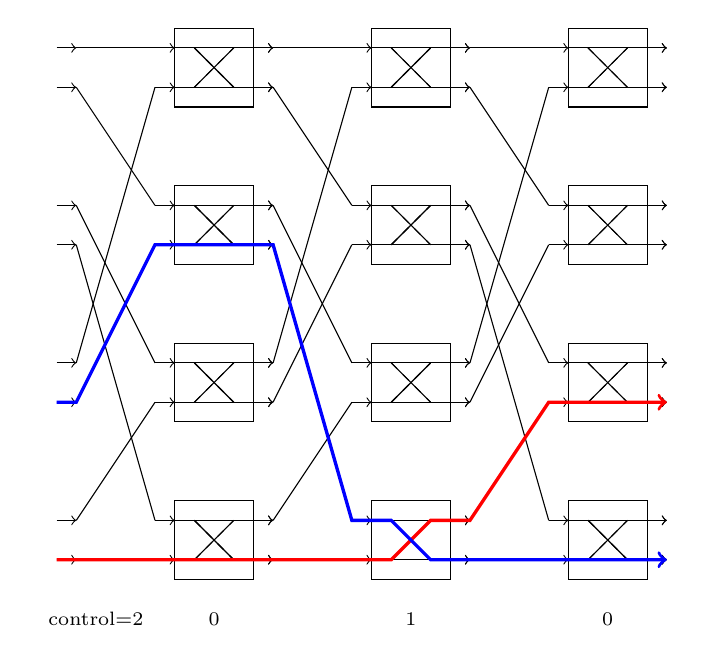
\begin{tikzpicture}[scale = .5]
            \foreach \i/\on in {0/0, 5/1, 10/0}{
                \foreach \j in {0, 4, 8, 12}{
                    \draw [shift={(\i,\j)}](-1,-1) rectangle (1,1);
                    \draw [shift={(\i,\j)}][->] (-1.5,-.5) -- (-1,-.5);
                    \draw [shift={(\i,\j)}][->] (-1.5,.5) -- (-1,.5);
                    \ifthenelse{\on=1}{
                        \draw [shift={(\i,\j)}](-.5,-.5) -- (.5,.5);
                        \draw [shift={(\i,\j)}](-.5,.5) -- (.5,-.5);
                        \draw [shift={(\i,\j)}] (-1,-.5) -- (-.5,-.5);
                        \draw [shift={(\i,\j)}] (-1,.5) -- (-.5,.5);
                        \draw [shift={(\i,\j)}][->] (.5,-.5) -- (1.5,-.5);
                        \draw [shift={(\i,\j)}][->] (.5,.5) -- (1.5,.5);
                        \draw [dashed,shift={(\i,\j)}](-.5,-.5) -- (.5,-.5);
                        \draw [dashed,shift={(\i,\j)}](-.5,.5) -- (.5,.5);
                    }{
                        \draw [shift={(\i,\j)}][->] (-1,-.5) -- (1.5,-.5);
                        \draw [shift={(\i,\j)}][->] (-1,.5) -- (1.5,.5);
                        \draw [dashed,shift={(\i,\j)}](-.5,-.5) -- (.5,.5);
                        \draw [dashed,shift={(\i,\j)}](-.5,.5) -- (.5,-.5);
                    }
                }
                \foreach \j/\k in {-.5/-.5,.5/3.5, 3.5/7.5, 4.5/11.5}{
                    \draw (\i-3.5, \j) -- (\i-1.5, \k);
                }
                \foreach \j/\k in {7.5/.5,8.5/4.5, 11.5/8.5, 12.5/12.5}{
                    \draw (\i-3.5, \j) -- (\i-1.5, \k);
                }
            }
            \foreach \i in {-.5,.5, 3.5,4.5, 7.5,8.5, 11.5,12.5}{
                \draw [->](-4,\i) -- (-3.5,\i);
            }
            \path[draw,red,very thick,->] (-4,-.5) -- (4.5,-.5) -- ++(1,1) -- ++(1,0) -- ++(2,3) -- ++(3,0);
            \path[draw,blue,very thick,->] (-4,3.5) -- ++(.5,0) -- ++(2,4) -- ++(3,0) -- ++(2,-7) -- ++(1,0) -- ++(1,-1) -- ++(6,0);
            \foreach [count=\c] \i in {-.5,.5, 3.5,4.5, 7.5,8.5, 11.5,12.5}{
                \FPeval{\z}{round(\c-1:0)};
                \node at (-4.5,\i) {\scriptsize \z};
                \node at (12,\i) {\scriptsize \z};
            }
            \node at (0,-2) {\scriptsize 0};
            \node at (5,-2) {\scriptsize 1};
            \node at (10,-2) {\scriptsize 0};
            \node at (-3,-2) {\scriptsize control=2};
        \end{tikzpicture}
        \caption{An 8-by-8 Omega network. We turn columns on or off to rotate between different routing configurations.}
        \label{fig:omega010}
    \end{figure}

    An Omega network consists of columns of Banyan switches~\cite{f-scratch:wu,f-scratch:lawrie}. A Banyan switch synthesizes to two multiplexers. In the ON state, the switch crosses data over to the opposite output port. As an illustrative example, the second column in Fig.~\ref{fig:omega010} only contains switches in the ON state. In the OFF state, the switch passes data straight to the corresponding output port. The first and last columns in Fig.~\ref{fig:omega010} only contain switches in the OFF state.

The Omega network has features that make it attractive in a multi-port memory design. If we switch whole columns of Banyan switches ON or OFF, we can easily determine where signals route by XORing the starting port index with the bits controlling the columns. For example, in Fig.~\ref{fig:omega010}, the control bits equal $010_2$ or 2 and input port 2 ($010_2$) routes to output port 0. Not coincidentally, the same configuration routes in reverse. Input port 0 routes to output port 2 and input port 2 routes to output port 0. This means the design can use identical control bits for both the receiving and sending Omega networks.

In the Omega multi-port memory design, the control for this network increments every clock cycle. As an example, input port 5 would connect to output port 5, then port 4, 7, 6, 1, etc., until it cycles around again. This means each input connects to each output an equal number of times.

\subsubsection{Linked List FIFO}
\label{sec:linkedfifo}
    \begin{figure}
        \center
        \begin{subfigure}{.4\linewidth}
        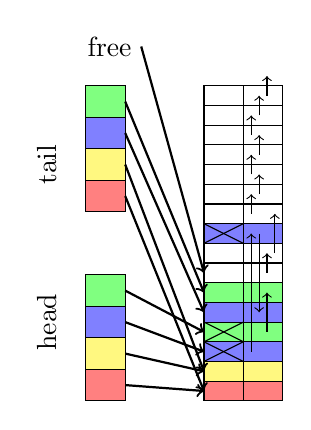
\begin{tikzpicture}
        \fill [red!50] (-.5,-2) rectangle (.5,-1.75);
        \fill [yellow!50] (-.5,-1.75) rectangle (.5,-1.5);
        \fill [blue!50] (-.5,-1.5) rectangle (.5,-1.25);
        \fill [blue!50] (-.5,-1) rectangle (.5,-.75);
        \fill [blue!50] (-.5,0) rectangle (.5,.25);
        \fill [green!50] (-.5,-1.25) rectangle (.5,-1);
        \fill [green!50] (-.5,-.5) rectangle (.5,-.75);
        \draw (-.5,-2) rectangle (0,2);
        \draw (0,-2) rectangle (.5,2);
        \foreach \i in {-1.75,-1.5,...,1.75}{
            \draw (-.5,\i) -- (.5,\i);
        }
        \node at (-2.5,-1)[rotate=90]{head};
        \node at (-2.5,1)[rotate=90]{tail};
        \node (f) at (-1.7,2.5) {free};
        \fill [red!50] (-2,-2) rectangle (-1.5,-1.6);
        \fill [yellow!50] (-2,-1.6) rectangle (-1.5,-1.2);
        \fill [blue!50] (-2,-1.2) rectangle (-1.5,-.8);
        \fill [green!50] (-2,-.8) rectangle (-1.5,-.4);
        \fill [red!50] (-2,.4) rectangle (-1.5,.8);
        \fill [yellow!50] (-2,.8) rectangle (-1.5,1.2);
        \fill [blue!50] (-2,1.2) rectangle (-1.5,1.6);
        \fill [green!50] (-2,1.6) rectangle (-1.5,2);
        \draw (-2,-2) rectangle (-1.5, -.4);
        \draw (-2,2) rectangle (-1.5, .4);
        \foreach \i in {-1.6,-1.2,-.8,.8,1.2,1.6}{
            \draw (-2,\i) -- (-1.5,\i);
        }
        \foreach[count=\i] \l/\h in {0/0,1/1,2/4,3/5}{
            \draw [thick,->] (-1.5,-1.8+\i*.4-.4) -- (-.5,\l*.25-1.875);
            \draw [thick,->] (-1.5,.6+\i*.4-.4) -- (-.5,\h*.25-1.875);
        }
        \draw (-.5,-1.5) -- (0,-1.25);
        \draw (-.5,-1.25) -- (0,-1.5);
        \draw (-.5,-1.25) -- (0,-1);
        \draw (-.5,-1) -- (0,-1.25);
        \draw (-.5,.25) -- (0,0);
        \draw (-.5,0) -- (0,.25);
        \draw [thick,->] (f.east) -- (-.5,-.375);
        \draw [->] (.1,-1.375) -- (.1,.125);
        \draw [->] (.2,.125) -- (.2,-.875);
        \draw [->] (.3,-.375) -- (.3,-.125);
        \draw [->] (.4,-.125) -- (.4,.375);
        \draw [->] (.3,-1.125) -- (.3,-.625);
        \foreach \i in {.375,.875,...,1.625}{
            \draw [->] (.1,\i) -- (.1,\i+.25);
            \draw [->] (.2,\i+.25) -- (.2,\i+.5);
        }
        \draw [->] (.3,1.875) -- (.3,2.125);

        \end{tikzpicture}
        \caption{Initial example}
        \label{fig:linked0}
    \end{subfigure}
        \begin{subfigure}{.4\linewidth}

        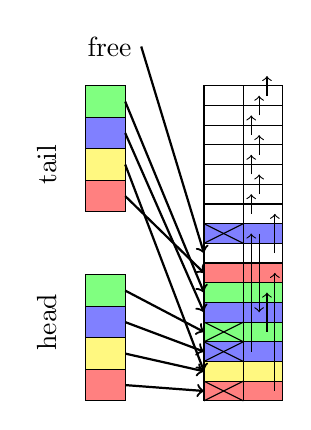
\begin{tikzpicture}
        \fill [red!50] (-.5,-2) rectangle (.5,-1.75);
        \fill [red!50] (-.5,-.5) rectangle (.5,-.25);
        \fill [yellow!50] (-.5,-1.75) rectangle (.5,-1.5);
        \fill [blue!50] (-.5,-1.5) rectangle (.5,-1.25);
        \fill [blue!50] (-.5,-1) rectangle (.5,-.75);
        \fill [blue!50] (-.5,0) rectangle (.5,.25);
        \fill [green!50] (-.5,-1.25) rectangle (.5,-1);
        \fill [green!50] (-.5,-.5) rectangle (.5,-.75);
        \draw (-.5,-2) rectangle (0,2);
        \draw (0,-2) rectangle (.5,2);
        \foreach \i in {-1.75,-1.5,...,1.75}{
            \draw (-.5,\i) -- (.5,\i);
        }
        \node at (-2.5,-1)[rotate=90]{head};
        \node at (-2.5,1)[rotate=90]{tail};
        \node (f) at (-1.7,2.5) {free};
        \fill [red!50] (-2,-2) rectangle (-1.5,-1.6);
        \fill [yellow!50] (-2,-1.6) rectangle (-1.5,-1.2);
        \fill [blue!50] (-2,-1.2) rectangle (-1.5,-.8);
        \fill [green!50] (-2,-.8) rectangle (-1.5,-.4);
        \fill [red!50] (-2,.4) rectangle (-1.5,.8);
        \fill [yellow!50] (-2,.8) rectangle (-1.5,1.2);
        \fill [blue!50] (-2,1.2) rectangle (-1.5,1.6);
        \fill [green!50] (-2,1.6) rectangle (-1.5,2);
        \draw (-2,-2) rectangle (-1.5, -.4);
        \draw (-2,2) rectangle (-1.5, .4);
        \foreach \i in {-1.6,-1.2,-.8,.8,1.2,1.6}{
            \draw (-2,\i) -- (-1.5,\i);
        }
        \foreach[count=\i] \l/\h in {0/6,1/1,2/4,3/5}{
            \draw [thick,->] (-1.5,-1.8+\i*.4-.4) -- (-.5,\l*.25-1.875);
            \draw [thick,->] (-1.5,.6+\i*.4-.4) -- (-.5,\h*.25-1.875);
        }
        \draw (-.5,-2) -- (0,-1.75);
        \draw (-.5,-1.75) -- (0,-2);
        \draw (-.5,-1.5) -- (0,-1.25);
        \draw (-.5,-1.25) -- (0,-1.5);
        \draw (-.5,-1.25) -- (0,-1);
        \draw (-.5,-1) -- (0,-1.25);
        \draw (-.5,.25) -- (0,0);
        \draw (-.5,0) -- (0,.25);
        \draw [thick,->] (f.east) -- (-.5,-.125);
        \draw [->] (.1,-1.375) -- (.1,.125);
        \draw [->] (.2,.125) -- (.2,-.875);
        \draw [->] (.4,-1.875) -- (.4,-.375);
        \draw [->] (.4,-.125) -- (.4,.375);
        \draw [->] (.3,-1.125) -- (.3,-.625);
        \foreach \i in {.375,.875,...,1.625}{
            \draw [->] (.1,\i) -- (.1,\i+.25);
            \draw [->] (.2,\i+.25) -- (.2,\i+.5);
        }
        \draw [->] (.3,1.875) -- (.3,2.125);

        \end{tikzpicture}
        \caption{First clock cycle}
        \label{fig:linked1}
    \end{subfigure}
        \begin{subfigure}{.4\linewidth}

        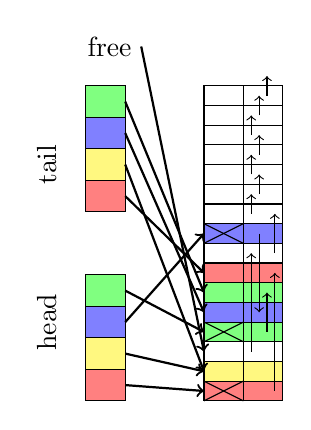
\begin{tikzpicture}
        \fill [red!50] (-.5,-2) rectangle (.5,-1.75);
        \fill [red!50] (-.5,-.5) rectangle (.5,-.25);
        \fill [yellow!50] (-.5,-1.75) rectangle (.5,-1.5);
        \fill [blue!50] (-.5,-1) rectangle (.5,-.75);
        \fill [blue!50] (-.5,0) rectangle (.5,.25);
        \fill [green!50] (-.5,-1.25) rectangle (.5,-1);
        \fill [green!50] (-.5,-.5) rectangle (.5,-.75);
        \draw (-.5,-2) rectangle (0,2);
        \draw (0,-2) rectangle (.5,2);
        \foreach \i in {-1.75,-1.5,...,1.75}{
            \draw (-.5,\i) -- (.5,\i);
        }
        \node at (-2.5,-1)[rotate=90]{head};
        \node at (-2.5,1)[rotate=90]{tail};
        \node (f) at (-1.7,2.5) {free};
        \fill [red!50] (-2,-2) rectangle (-1.5,-1.6);
        \fill [yellow!50] (-2,-1.6) rectangle (-1.5,-1.2);
        \fill [blue!50] (-2,-1.2) rectangle (-1.5,-.8);
        \fill [green!50] (-2,-.8) rectangle (-1.5,-.4);
        \fill [red!50] (-2,.4) rectangle (-1.5,.8);
        \fill [yellow!50] (-2,.8) rectangle (-1.5,1.2);
        \fill [blue!50] (-2,1.2) rectangle (-1.5,1.6);
        \fill [green!50] (-2,1.6) rectangle (-1.5,2);
        \draw (-2,-2) rectangle (-1.5, -.4);
        \draw (-2,2) rectangle (-1.5, .4);
        \foreach \i in {-1.6,-1.2,-.8,.8,1.2,1.6}{
            \draw (-2,\i) -- (-1.5,\i);
        }
        \foreach[count=\i] \l/\h in {0/6,1/1,8/4,3/5}{
            \draw [thick,->] (-1.5,-1.8+\i*.4-.4) -- (-.5,\l*.25-1.875);
            \draw [thick,->] (-1.5,.6+\i*.4-.4) -- (-.5,\h*.25-1.875);
        }
        \draw (-.5,-2) -- (0,-1.75);
        \draw (-.5,-1.75) -- (0,-2);
        \draw (-.5,-1.25) -- (0,-1);
        \draw (-.5,-1) -- (0,-1.25);
        \draw (-.5,.25) -- (0,0);
        \draw (-.5,0) -- (0,.25);
        \draw [thick,->] (f.east) -- (-.5,-1.375);
        \draw [->] (.1,-1.375) -- (.1,-.125);
        \draw [->] (.2,.125) -- (.2,-.875);
        \draw [->] (.4,-1.875) -- (.4,-.375);
        \draw [->] (.4,-.125) -- (.4,.375);
        \draw [->] (.3,-1.125) -- (.3,-.625);
        \foreach \i in {.375,.875,...,1.625}{
            \draw [->] (.1,\i) -- (.1,\i+.25);
            \draw [->] (.2,\i+.25) -- (.2,\i+.5);
        }
        \draw [->] (.3,1.875) -- (.3,2.125);

        \end{tikzpicture}
        \caption{Second clock cycle}
        \label{fig:linked2}
    \end{subfigure}
        \begin{subfigure}{.4\linewidth}
        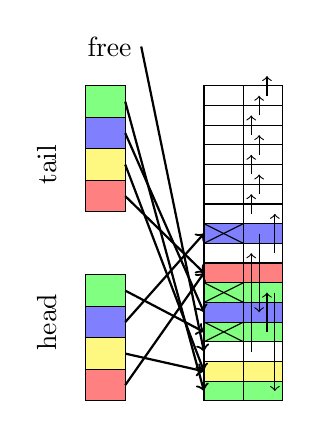
\begin{tikzpicture}
        \fill [green!50] (-.5,-2) rectangle (.5,-1.75);
        \fill [red!50] (-.5,-.5) rectangle (.5,-.25);
        \fill [yellow!50] (-.5,-1.75) rectangle (.5,-1.5);
        \fill [blue!50] (-.5,-1) rectangle (.5,-.75);
        \fill [blue!50] (-.5,0) rectangle (.5,.25);
        \fill [green!50] (-.5,-1.25) rectangle (.5,-1);
        \fill [green!50] (-.5,-.5) rectangle (.5,-.75);
        \draw (-.5,-2) rectangle (0,2);
        \draw (0,-2) rectangle (.5,2);
        \foreach \i in {-1.75,-1.5,...,1.75}{
            \draw (-.5,\i) -- (.5,\i);
        }
        \node at (-2.5,-1)[rotate=90]{head};
        \node at (-2.5,1)[rotate=90]{tail};
        \node (f) at (-1.7,2.5) {free};
        \fill [red!50] (-2,-2) rectangle (-1.5,-1.6);
        \fill [yellow!50] (-2,-1.6) rectangle (-1.5,-1.2);
        \fill [blue!50] (-2,-1.2) rectangle (-1.5,-.8);
        \fill [green!50] (-2,-.8) rectangle (-1.5,-.4);
        \fill [red!50] (-2,.4) rectangle (-1.5,.8);
        \fill [yellow!50] (-2,.8) rectangle (-1.5,1.2);
        \fill [blue!50] (-2,1.2) rectangle (-1.5,1.6);
        \fill [green!50] (-2,1.6) rectangle (-1.5,2);
        \draw (-2,-2) rectangle (-1.5, -.4);
        \draw (-2,2) rectangle (-1.5, .4);
        \foreach \i in {-1.6,-1.2,-.8,.8,1.2,1.6}{
            \draw (-2,\i) -- (-1.5,\i);
        }
        \foreach[count=\i] \l/\h in {6/6,1/1,8/4,3/0}{
            \draw [thick,->] (-1.5,-1.8+\i*.4-.4) -- (-.5,\l*.25-1.875);
            \draw [thick,->] (-1.5,.6+\i*.4-.4) -- (-.5,\h*.25-1.875);
        }
        \draw (-.5,-.75) -- (0,-.5);
        \draw (-.5,-.5) -- (0,-.75);
        \draw (-.5,-1.25) -- (0,-1);
        \draw (-.5,-1) -- (0,-1.25);
        \draw (-.5,.25) -- (0,0);
        \draw (-.5,0) -- (0,.25);
        \draw [thick,->] (f.east) -- (-.5,-1.375);
        \draw [->] (.1,-1.375) -- (.1,-.125);
        \draw [->] (.2,.125) -- (.2,-.875);
        \draw [->] (.4,-.625) -- (.4,-1.875);
        \draw [->] (.4,-.125) -- (.4,.375);
        \draw [->] (.3,-1.125) -- (.3,-.625);
        \foreach \i in {.375,.875,...,1.625}{
            \draw [->] (.1,\i) -- (.1,\i+.25);
            \draw [->] (.2,\i+.25) -- (.2,\i+.5);
        }
        \draw [->] (.3,1.875) -- (.3,2.125);

        \end{tikzpicture}
        \caption{Third clock cycle}
        \label{fig:linked3}
    \end{subfigure}
        \caption{A linked list FIFO during 3 clock cycles of operation}
        \label{fig:linkedfifo}
    \end{figure}
    The partnering hardware structure, the linked list FIFO (Fig.~\ref{fig:linkedfifo}), contains several internal FIFOs with no predefined space in a single RAM. Similar to a software linked list, there exists a free pointer that points to the beginning of the free space linked list. Linked list FIFOs have previously seen use in multi-core CPU~\cite{f-scratch:bell} and FPGA~\cite{f-scratch:nikologiannis} designs.

    Due to the linking pointers, the size of the RAM now needs $O(NlogN)$ space to store $N$ elements. However $logN$ grows slowly. For example, data stored in a 64-bit wide by 1024 deep RAM would need an additional 11-bit wide by 1024 deep RAM for the linking pointers. An illustrative example of the linked list FIFO is shown in in Fig.~\ref{fig:linkedfifo}, which uses a 16 deep RAM and 4 FIFOs.

    In the initial state (\figurename~\ref{fig:linked0}), the red and yellow FIFOs have no messages. The blue FIFO has two messages. And, the green FIFO has one message. However, every FIFO reserves one space for the next incoming value. This limits the total available space in the linked list FIFO to $TOTAL\_DEPTH-FIFO\_COUNT$.

    \begin{itemize}
        \item On the first clock cycle (Fig.~\ref{fig:linked1}), the linked list FIFO receives a push containing a red message. The new red message gets stored in the reserved space at the tail of the red linked list. The free linked list pops one space. That space gets pushed on to the red linked list.

        \item On the second clock cycle (Fig.~\ref{fig:linked2}), the linked list FIFO receives a pop for a blue message. A blue message gets popped from the head of the blue linked list. The newly freed space gets pushed on to the free linked list.

        \item On the third clock cycle (Fig.~\ref{fig:linked3}), the linked list receives a pop for a red message and a push for a green message. In this case the space that the red message was popped from gets pushed onto the green linked list. The free space linked list stays the same.
    \end{itemize}

\subsection{Reorder Queue}
    \begin{figure}
        \center
        \begin{subfigure}{.32\linewidth}
            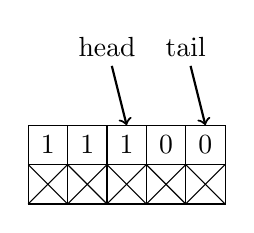
\begin{tikzpicture}
                \draw (0,0) rectangle (2.5,1);
                \draw (0,.5) -- (2.5,.5);
            \foreach \i in {.5,1,...,2}{
                \draw (\i,0) -- (\i,1);
            }
            \foreach \i/\j/\k in {0/1/0,1/1/0,2/1/1,3/0/0,4/0/0}{
                \node at (\i*.5+.25,.75) {\j};
                \ifthenelse{\k=1}{
                    \draw (\i*.5,0) -- (\i*.5+.5,.5);
                    \draw (\i*.5,.5) -- (\i*.5+.5,0);
                }{};
            }
            \node at (1,2) (b) {head};
            \node at (2,2) (e) {tail};
            \draw [thick,->] (b) -- (1.25,1);
            \draw [thick,->] (e) -- (2.25,1);

            \end{tikzpicture}
            \caption{Initial example}
            \label{fig:reorder0}
        \end{subfigure}
        \begin{subfigure}{.32\linewidth}
            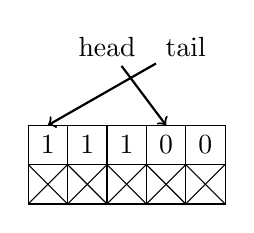
\begin{tikzpicture}
                \draw (0,0) rectangle (2.5,1);
                \draw (0,.5) -- (2.5,.5);
            \foreach \i in {.5,1,...,2}{
                \draw (\i,0) -- (\i,1);
            }
            \foreach \i/\j/\k in {0/1/0,1/1/0,2/1/0,3/0/0,4/0/0}{
                \node at (\i*.5+.25,.75) {\j};
                \ifthenelse{\k=1}{
                    \draw (\i*.5,0) -- (\i*.5+.5,.5);
                    \draw (\i*.5,.5) -- (\i*.5+.5,0);
                }{};
            }
            \node at (1,2) (b) {head};
            \node at (2,2) (e) {tail};
            \draw [thick,->] (b) -- (1.75,1);
            \draw [thick,->] (e) -- (.25,1);

            \end{tikzpicture}
            \caption{First clock cycle}
            \label{fig:reorder1}
        \end{subfigure}
        \begin{subfigure}{.32\linewidth}
            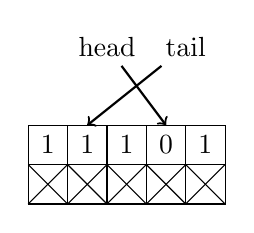
\begin{tikzpicture}
                \draw (0,0) rectangle (2.5,1);
                \draw (0,.5) -- (2.5,.5);
            \foreach \i in {.5,1,...,2}{
                \draw (\i,0) -- (\i,1);
            }
            \foreach \i/\j/\k in {0/1/0,1/1/0,2/1/0,3/0/0,4/1/1}{
                \node at (\i*.5+.25,.75) {\j};
                \ifthenelse{\k=1}{
                    \draw (\i*.5,0) -- (\i*.5+.5,.5);
                    \draw (\i*.5,.5) -- (\i*.5+.5,0);
                }{};
            }
            \node at (1,2) (b) {head};
            \node at (2,2) (e) {tail};
            \draw [thick,->] (b) -- (1.75,1);
            \draw [thick,->] (e) -- (.75,1);

            \end{tikzpicture}
            \caption{Second clock cycle}
            \label{fig:reorder2}
        \end{subfigure}
        \begin{subfigure}{.32\linewidth}
            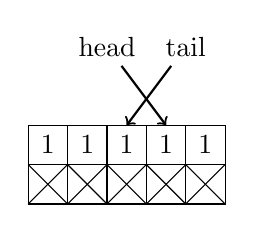
\begin{tikzpicture}
                \draw (0,0) rectangle (2.5,1);
                \draw (0,.5) -- (2.5,.5);
            \foreach \i in {.5,1,...,2}{
                \draw (\i,0) -- (\i,1);
            }
            \foreach \i/\j/\k in {0/1/0,1/1/0,2/1/0,3/1/1,4/1/1}{
                \node at (\i*.5+.25,.75) {\j};
                \ifthenelse{\k=1}{
                    \draw (\i*.5,0) -- (\i*.5+.5,.5);
                    \draw (\i*.5,.5) -- (\i*.5+.5,0);
                }{};
            }
            \node at (1,2) (b) {head};
            \node at (2,2) (e) {tail};
            \draw [thick,->] (b) -- (1.75,1);
            \draw [thick,->] (e) -- (1.25,1);

            \end{tikzpicture}
            \caption{Third clock cycle}
            \label{fig:reorder3}
        \end{subfigure}
        \begin{subfigure}{.32\linewidth}
            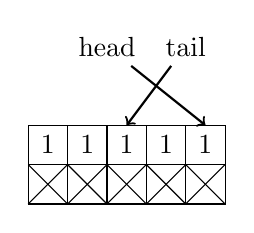
\begin{tikzpicture}
                \draw (0,0) rectangle (2.5,1);
                \draw (0,.5) -- (2.5,.5);
            \foreach \i in {.5,1,...,2}{
                \draw (\i,0) -- (\i,1);
            }
            \foreach \i/\j/\k in {0/1/0,1/1/0,2/1/0,3/1/0,4/1/1}{
                \node at (\i*.5+.25,.75) {\j};
                \ifthenelse{\k=1}{
                    \draw (\i*.5,0) -- (\i*.5+.5,.5);
                    \draw (\i*.5,.5) -- (\i*.5+.5,0);
                }{};
            }
            \node at (1,2) (b) {head};
            \node at (2,2) (e) {tail};
            \draw [thick,->] (b) -- (2.25,1);
            \draw [thick,->] (e) -- (1.25,1);

            \end{tikzpicture}
            \caption{Fourth clock cycle}
            \label{fig:reorder4}
        \end{subfigure}
        \begin{subfigure}{.32\linewidth}
            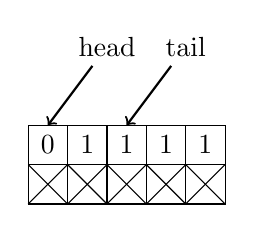
\begin{tikzpicture}
                \draw (0,0) rectangle (2.5,1);
                \draw (0,.5) -- (2.5,.5);
            \foreach \i in {.5,1,...,2}{
                \draw (\i,0) -- (\i,1);
            }
            \foreach \i/\j/\k in {0/0/1,1/1/0,2/1/0,3/1/0,4/1/0}{
                \node at (\i*.5+.25,.75) {\j};
                \ifthenelse{\k=1}{
                    \draw (\i*.5,0) -- (\i*.5+.5,.5);
                    \draw (\i*.5,.5) -- (\i*.5+.5,0);
                }{};
            }
            \node at (1,2) (b) {head};
            \node at (2,2) (e) {tail};
            \draw [thick,->] (b) -- (.25,1);
            \draw [thick,->] (e) -- (1.25,1);

            \end{tikzpicture}
            \caption{Fifth clock cycle}
            \label{fig:reorder5}
        \end{subfigure}
        %\input{fig/reorder.tex}
        \caption{Reorder queue example.}
        \label{fig:reorder}
    \end{figure}

    The buffering in both designs ensures relatively high throughput, however, this buffering causes a problem for both memories, as read responses from different banks from the same port may come back out of order. Although out of order reads do not always cause an issue, to alleviate this issue we add reorder queues (Fig.~\ref{fig:reordermemory}) to both multi-port memory designs.

    A reorder queue behaves similarly to a FIFO. However, some of the values in between the head and tail pointer exist ``in flight'' and not at the reorder queue memory. The reorder queue keeps track of the presence of messages with a bit array (a 1-bit wide RAM).

    \figurename~\ref{fig:reorder} shows an example with 5 clock cycles of operation. In the initial state (Fig.~\ref{fig:reorder0}), the reorder queue has one present message and one in flight message.

    \begin{itemize}
        \item On the first clock cycle (Fig.~\ref{fig:reorder1}), the present message at the head gets popped from the queue. A new message increments the tail, but the message remains in flight until it arrives at the reorder queue.

        \item On the second clock cycle (Fig.~\ref{fig:reorder2}), a new message arrives at the reorder queue, however, it does not arrive at the head of the queue so no message can get popped.

        \item On the third clock cycle (Fig.~\ref{fig:reorder3}), a message arrives at the head of the reorder queue.

        \item On the fourth clock cycle (Fig.~\ref{fig:reorder4}), this message at the head of the reorder queue gets popped. If the reorder queue did not exist, the message that appeared on clock cycle 2 would have reached the output first even though it was sent later.

        \item On the fifth clock cycle (\figurename~\ref{fig:reorder5}), a message arrives. However, the meaning of 1 or 0 in the 1-bit RAM switched after the pointers wrapped around the end of the RAM. Instead of 1 meaning present, 1 now means in flight. This semantic flipping allows the use of only one write port on the 1-bit RAM (instead of two if the bits flipped after popping a message), saving on memory-related resources. 
    \end{itemize}

    \begin{figure}
        \center
        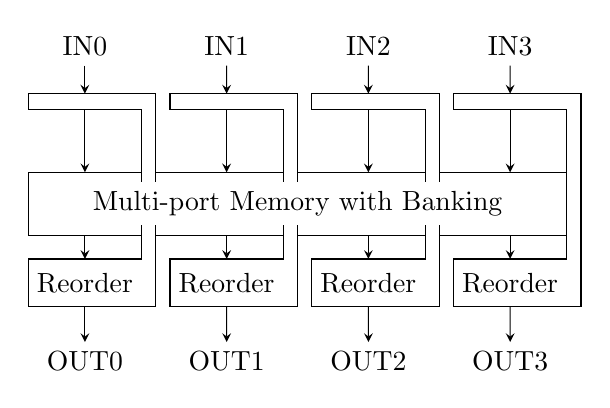
\begin{tikzpicture}[xscale=1.8]
            \draw (-.4,-1.6) rectangle (3.4,-2.4);
            \foreach \x in {0,1,...,3}{
                \node at (\x,0)(in){IN\x};
                \node at (\x,-4)(out){OUT\x};
                \draw[xshift=\x cm - .1 cm,fill=white](-.3,-.6) -- (-.3,-.8) -- (.5,-.8) -- (.5,-2.7) -- (-.3,-2.7) -- (-.3,-3.3) -- (.6,-3.3) -- (.6, -.6) -- cycle;
                \node at (\x, -3){Reorder};
                \path[draw,>=stealth,->] (in) -- (\x,-.6);
                \path[draw,>=stealth,->] (\x,-.8) -- (\x,-1.6);
                \path[draw,>=stealth,->] (\x,-2.4) -- (\x,-2.7);
                \path[draw,>=stealth,->] (\x,-3.3) -- (out);
            }
            \node[fill=white] at (1.5,-2){Multi-port Memory with Banking};
        \end{tikzpicture}
        \caption{A reorder queue tags incoming read requests with an ID that allows the reorder queue to know the correct order of the read responses.}
        \label{fig:reordermemory}
    \end{figure}

\section{Evaluation Methodology}
\label{sec:evaluation}
    We implemented a small resource and a large resource version of each memory. The small version does not use RAM blocks for buffering, and limits linked list FIFOs and reorder queues to a depth of 64. The large version does use RAM blocks for buffering and limits these memories to a depth of 512. However, in both cases we limit the depth of the FIFOs in the fully-connected interconnect network to 32 since the number of FIFOs in it grows by $O(N^2)$.

    For synthesis we used Xilinx Synthesis Tools (XST) and targeted the Xilinx Virtex-7 V2000T. The V2000T has a relatively large number of logic blocks and RAM blocks, which helps us push the limits of these designs. These designs should also work well on Altera FPGAs, given the commonalities between the devices. Both Xilinx and Altera use a base depth of 32 for distributed RAM and a base depth of 512 for RAM blocks.

    We used the ModelSim logic simulator to evaluate the performance of each configuration. The testbench used for evaluation consists of four benchmarks. Each benchmark tests the read performance of different memory access patterns: {\em sequential}, {\em random}, {\em congested}, or {\em segregated}.

    The {\em sequential} benchmark begins by sending a read request to memory address 0 on each port. On the next clock cycle each port requests data from memory address 1. This continues unless a port stalls. On a stall, the memory address of that port does not increment until the memory resolves the stall.

    The {\em random} benchmark begins by sending a read request to a random memory address on each port. On the next clock cycle, every port gets a new random memory address to read from. This continues until the end of the benchmark.

    The {\em congested} benchmark begins by sending a read request to memory address 0 on each port. On  subsequent clock cycles, the memory address does not change. This results in all the ports attempting to access the same memory bank. The purpose of this benchmark is to demonstrate the worst-case performance for any type of multi-port memory with banking, including our designs.

    The {\em segregated} benchmark begins by sending a read request to memory address $i$ on each port, where $i$ equals the index of the requested port. This address does not change on subsequent clock cycles. This results in all the banks receiving an equal number of requests. However, unlike the sequential and random benchmarks, there exists an uneven distribution of requests among all $N^2$ port to bank connections.

    We calculate the throughput of a given benchmark by measuring the ratio of read requests to potential read requests. If no stalls occur, the throughput equals 100\%. We calculate the latency by measuring the number of clock cycles between the last read request and the last read response. 
    %Other measures of latency exist, but none stood out as a superior way to measure latency.

%\begin{table}
%    \center
%    \caption{Analysis of multi-port memories}
%    \label{tbl:resources0}
%\begin{threeparttable}
%\begin{tabular}{|l|l|l|l|l|l|l|l|l|l|l|}
%\hline
%&Ports & & 4 & 8 & 16 & 32 & 64 & 128 & 256 \\
%&Memory Space & &  16KB & 32KB & 64KB & 128KB & 256KB & 512KB & 1MB \\
%\hline
%\multirow{26}{*}{\tikz \node at (0,0) [rotate=90]{Linked List FIFO and Reorder Queue Depth set to 64};} & & \multicolumn{8}{|c|}{Standard Multi-port Memory}\\
%\cline{2-10}
%&\multirow{4}{*}{\shortstack[l]{Resource\\Utilization\\Virtex 7\\ V2000T\tnote{2}}} & Registers & 4K & 14K & 50K & 190K & 728K & \cellcolor{gray} & \cellcolor{gray} \\
%&                                                                          & LUTs      & 5.7K & 18K & 61K & 241K & 906K & \cellcolor{gray} & \cellcolor{gray} \\
%&& BlockRAM  & 4 & 8 & 16 & 32 & 64  &\cellcolor{gray}  & \cellcolor{gray} \\
%& & Clock frequency & 345Mhz & 313Mhz & 256Mhz & 273Mhz & 230Mhz   & \cellcolor{gray} & \cellcolor{gray} \\
%\cline{2-10}
%&Sequential & Throughput & 100\% & 100\% & 100\% & 100\% & 50\% & \cellcolor{gray} & \cellcolor{gray} \\
%& & Latency \tnote{1} & 16 & 20 & 36 & 64 & 128  & \cellcolor{gray} & \cellcolor{gray} \\
%&Random & Throughput & 97\% & 93\% & 88\% & 72\% & 49\% & \cellcolor{gray} & \cellcolor{gray} \\
%& & Latency \tnote{1} & 66 & 65 & 85 & 97 & 144& \cellcolor{gray} & \cellcolor{gray} \\
%&Congested & Throughput & 25\% & 13\% & 6\% & 3\% & 2\% & \cellcolor{gray} & \cellcolor{gray} \\
%& & Latency \tnote{1} & 105 & 230 & 490 & 1034 & 2780 & \cellcolor{gray} & \cellcolor{gray} \\
%&Segregated & Throughput & 100\% & 100\% & 100\% & 100\% & 100\% & \cellcolor{gray} & \cellcolor{gray} \\
%& & Latency \tnote{1} & 16 & 24 & 34 & 63 & 61 & \cellcolor{gray} & \cellcolor{gray} \\
%\cline{2-10}
%& & \multicolumn{8}{|c|}{Omega Multi-port Memory} \\
%\cline{2-10}
%&\multirow{4}{*}{\shortstack[l]{Resource\\Utilization\\Virtex 7\\ V2000T\tnote{2}}}& Registers & 3K & 9K & 22K & 53K & \cellcolor{gray} & \cellcolor{gray} & \cellcolor{gray} \\
%&                                                                      & LUTs      & 5K & 11K & 24K & 53K & \cellcolor{gray} & \cellcolor{gray} & \cellcolor{gray} \\
%&& BlockRAM  & 4 & 8 & 16 & 32 & \cellcolor{gray} & \cellcolor{gray} & \cellcolor{gray} \\
%&& Clock frequency & 258Mhz & 257Mhz & 260Mhz & 262Mhz & \cellcolor{gray} & \cellcolor{gray} & \cellcolor{gray} \\
%\cline{2-10}
%&Sequential & Throughput & 100\%  & 100\% & 100\% & 100\% & \cellcolor{gray} & \cellcolor{gray} & \cellcolor{gray} \\
%&& Latency \tnote{1} & 17 & 25 & 37 & 56 & \cellcolor{gray} & \cellcolor{gray} & \cellcolor{gray} \\
%&Random & Throughput & 94\% & 83\% & 68\% & 52\% & \cellcolor{gray} & \cellcolor{gray} & \cellcolor{gray} \\
%& & Latency \tnote{1} & 72 & 110 & 131 & 193 & \cellcolor{gray} & \cellcolor{gray} & \cellcolor{gray} \\
%&Congested & Throughput & 25\% & 13\% & 6\% & 3\% & \cellcolor{gray} & \cellcolor{gray} & \cellcolor{gray} \\
%& & Latency \tnote{1} & 250 & 462 & 786 & 1046 & \cellcolor{gray} & \cellcolor{gray} & \cellcolor{gray} \\
%&Segregated & Throughput & 25\% & 13\% & 6\% & 3\% & \cellcolor{gray} & \cellcolor{gray} & \cellcolor{gray} \\
%& & Latency \tnote{1} & 247 & 461 & 756 & 1043 & \cellcolor{gray} & \cellcolor{gray} & \cellcolor{gray} \\
%\hline
%\end{tabular}
%\end{threeparttable}
%\end{table}
\begin{table*}
    \center
    \caption{Analysis of the two multi-port memory designs.}
    \label{tbl:resources}
\begin{threeparttable}
\begin{tabular}{|l|l|l|l|l|l|l|l|l|l|l|}
\hline
&Ports & & 4 & 8 & 16 & 32 & 64 & 128 & 256 \\
&Memory Space & &  16KB & 32KB & 64KB & 128KB & 256KB & 512KB & 1MB \\
\hline
\multirow{26}{*}{\tikz \node at (0,0) [rotate=90]{Linked List FIFO and Reorder Queue Depth set to 64};} & & \multicolumn{8}{|c|}{Fully-connected Multi-port Memory}\\
\cline{2-10}
&\multirow{4}{*}{\shortstack[l]{Resource\\Utilization\\Virtex 7\\ V2000T\tnote{2}}} & Registers & 4K & 14K & 50K & 190K & 728K & \cellcolor{gray} & \cellcolor{gray} \\
&                                                                          & LUTs      & 5.7K & 18K & 61K & 241K & 906K & \cellcolor{gray} & \cellcolor{gray} \\
&& BlockRAM  & 4 & 8 & 16 & 32 & 64  &\cellcolor{gray}  & \cellcolor{gray} \\
& & Clock frequency & 345Mhz & 313Mhz & 256Mhz & 273Mhz & 230Mhz   & \cellcolor{gray} & \cellcolor{gray} \\
\cline{2-10}
&Sequential & Throughput & 100\% & 100\% & 100\% & 100\% & 50\% & \cellcolor{gray} & \cellcolor{gray} \\
& & Latency \tnote{1} & 16 & 20 & 36 & 64 & 128  & \cellcolor{gray} & \cellcolor{gray} \\
&Random & Throughput & 97\% & 93\% & 88\% & 72\% & 49\% & \cellcolor{gray} & \cellcolor{gray} \\
& & Latency \tnote{1} & 66 & 65 & 85 & 97 & 144& \cellcolor{gray} & \cellcolor{gray} \\
&Congested & Throughput & 25\% & 13\% & 6\% & 3\% & 2\% & \cellcolor{gray} & \cellcolor{gray} \\
& & Latency \tnote{1} & 105 & 230 & 490 & 1034 & 2780 & \cellcolor{gray} & \cellcolor{gray} \\
&Segregated & Throughput & 100\% & 100\% & 100\% & 100\% & 100\% & \cellcolor{gray} & \cellcolor{gray} \\
& & Latency \tnote{1} & 16 & 24 & 34 & 63 & 61 & \cellcolor{gray} & \cellcolor{gray} \\
\cline{2-10}
& & \multicolumn{8}{|c|}{Omega Multi-port Memory} \\
\cline{2-10}
&\multirow{4}{*}{\shortstack[l]{Resource\\Utilization\\Virtex 7\\ V2000T\tnote{2}}}& Registers & 3K & 9K & 22K & 53K & \cellcolor{gray} & \cellcolor{gray} & \cellcolor{gray} \\
&                                                                      & LUTs      & 5K & 11K & 24K & 53K & \cellcolor{gray} & \cellcolor{gray} & \cellcolor{gray} \\
&& BlockRAM  & 4 & 8 & 16 & 32 & \cellcolor{gray} & \cellcolor{gray} & \cellcolor{gray} \\
&& Clock frequency & 258Mhz & 257Mhz & 260Mhz & 262Mhz & \cellcolor{gray} & \cellcolor{gray} & \cellcolor{gray} \\
\cline{2-10}
&Sequential & Throughput & 100\%  & 100\% & 100\% & 100\% & \cellcolor{gray} & \cellcolor{gray} & \cellcolor{gray} \\
&& Latency \tnote{1} & 17 & 25 & 37 & 56 & \cellcolor{gray} & \cellcolor{gray} & \cellcolor{gray} \\
&Random & Throughput & 94\% & 83\% & 68\% & 52\% & \cellcolor{gray} & \cellcolor{gray} & \cellcolor{gray} \\
& & Latency \tnote{1} & 72 & 110 & 131 & 193 & \cellcolor{gray} & \cellcolor{gray} & \cellcolor{gray} \\
&Congested & Throughput & 25\% & 13\% & 6\% & 3\% & \cellcolor{gray} & \cellcolor{gray} & \cellcolor{gray} \\
& & Latency \tnote{1} & 250 & 462 & 786 & 1046 & \cellcolor{gray} & \cellcolor{gray} & \cellcolor{gray} \\
&Segregated & Throughput & 25\% & 13\% & 6\% & 3\% & \cellcolor{gray} & \cellcolor{gray} & \cellcolor{gray} \\
& & Latency \tnote{1} & 247 & 461 & 756 & 1043 & \cellcolor{gray} & \cellcolor{gray} & \cellcolor{gray} \\
\hline
\hline
\multirow{26}{*}{\tikz \node at (0,0) [rotate=90]{Linked List FIFO and Reorder Queue Depth set to 512};} & & \multicolumn{8}{|c|}{Fully-connected Multi-port Memory}\\
\cline{2-10}

&\multirow{4}{*}{\shortstack[l]{Resource\\Utilization\\Virtex 7\\ V2000T\tnote{2}}}& Registers & 4.2K & 14K & 50K & 191K &  744K & \cellcolor{gray} & \cellcolor{gray} \\
&& LUTs      & 5.3K & 17K & 60K & 241K & 928K & \cellcolor{gray} & \cellcolor{gray} \\
&& BlockRAM  & 7 & 13 & 25 & 48 & 96 & \cellcolor{gray} & \cellcolor{gray} \\
& & Clock frequency & 352Mhz & 315Mhz & 253Mhz & 271Mhz & 230Mhz & \cellcolor{gray} & \cellcolor{gray} \\
\cline{2-10}
&Sequential & Throughput & 100\% & 100\% & 100\% & 100\% & 100\% & \cellcolor{gray} & \cellcolor{gray} \\
& & Latency \tnote{1} & 16 & 20 & 36 & 68 & 100 & \cellcolor{gray} & \cellcolor{gray} \\
&Random & Throughput & 96\% & 95\% & 94\% & 99\% & 98\% & \cellcolor{gray} & \cellcolor{gray} \\
& & Latency \tnote{1} & 134 & 296 & 512 & 553 & 616 & \cellcolor{gray} & \cellcolor{gray} \\
&Congested & Throughput & 25\% & 13\% & 6\% & 3\% & 2\% & \cellcolor{gray} & \cellcolor{gray} \\
& & Latency \tnote{1} & 105 & 231 & 491 & 1019 & 2750 & \cellcolor{gray} & \cellcolor{gray} \\
&Segregated & Throughput & 100\% & 100\% & 100\% & 100\% & 100\% & \cellcolor{gray} & \cellcolor{gray} \\
& & Latency \tnote{1} & 16 & 23 & 38 & 61 & 63 & \cellcolor{gray} & \cellcolor{gray} \\
\cline{2-10}
& & \multicolumn{8}{|c|}{Omega Multi-port Memory}\\
\cline{2-10}
&\multirow{4}{*}{\shortstack[l]{Resource\\Utilization\\Virtex 7\\ V2000T\tnote{2}}}& Registers & 3.0K & 8.4K & 23K & 53K & 125K & 300K & 677K \\
&& LUTs      & 7.3K & 16K & 36K & 77K & 163K & 345K & 746K \\
&& BlockRAM  & 9 & 17 & 32 & 65 & 129 & 257 & 513 \\
& & Clock frequency & 234Mhz & 234Mhz & 230Mhz & 230Mhz & 225Mhz & 202Mhz & 175Mhz    \\
\cline{2-10}
&Sequential & Throughput & 100\% & 100\% & 100\% & 100\% & 100\% & 100\% & 100\% \\
& & Latency \tnote{1} & 17 & 25 & 37 & 57 & 93 & 161 & 293 \\
&Random & Throughput & 100\% & 99\% & 96\% & 89\% & 78\% & 63\% & 48\% \\
& & Latency \tnote{1} & 312 & 580 & 566 & 751 & 1182 & 1397 & 2072 \\
&Congested & Throughput & 25\% & 13\% & 6\% & 3\% & 2\% & 1\% & 0.4\% \\
& & Latency \tnote{1} & 2040 & 4046 & 7954 & 15351 & 28698 & 49182 & 65556 \\
&Segregated & Throughput & 25\% & 13\% & 6\% & 3\% & 2\% & 1\% & 0.4\% \\
& & Latency \tnote{1} & 2037 & 4039 & 79530 & 15331 & 28593 & 49174 & 65388 \\
\hline
\end{tabular}
\begin{tablenotes}
\item[1] This measures the number of clock cycles between the end of the benchmark and when the last response of the last request gets received. In the worst case scenario several FIFOs queue data that has to wait for access to the same bank.
\item[2] This particular chip has 2.4M registers, 1.2M LUTs and 1.3K RAM blocks.
\end{tablenotes}
\end{threeparttable}
\end{table*}



\section{Results and Analysis}
\label{sec:analysis}
\begin{figure}[t]
    \center
    \begin{tikzpicture}[xscale=.19,yscale=.07]
        \tikzstyle{blueSquare}=[draw, rectangle, fill=blue, inner sep =2.5pt];
        \tikzstyle{redCircle}=[draw, circle, fill=red, inner sep =2.1pt];
        \tikzstyle{greenDiamond}=[draw, diamond, fill=green, inner sep =1.8pt];
        \tikzstyle{blackTriangle}=[draw, regular polygon, regular polygon sides=3, fill=black, inner sep =1.6pt];
        \draw [->] (0,0) -- (40,0);
        \draw [->] (0,0) -- (0,100);
        \foreach \i in {4,8,16,32}{
            \draw (\i,1) -- (\i,-1)node[anchor=20,rotate=60]{\i};
        }
        \foreach \y in {20,40,...,80}{
            \FPeval{\v}{round(\y*2.5:0)};
            \draw (.4,\y) -- (-.4,\y)node[anchor=south,rotate=90]{\v K};
        }
        \node at (20, -10) {Ports};
        \node at (-4,50) [rotate=90]{LUTs/Registers};
\foreach \xa/\ya/\xb/\yb in {4/4.1/8/14.0,8/14.0/16/50.0,16/50.0/32/190.0}{
    \draw [thick, red] (\xa,\ya/2.5) -- (\xb,\yb/2.5);
}
\foreach \xa/\ya/\xb/\yb in {4/5.7/8/18.0,8/18.0/16/61.0,16/61.0/32/241.0}{
    \draw [thick, blue] (\xa,\ya/2.5) -- (\xb,\yb/2.5);
}
\foreach \xa/\ya/\xb/\yb in {4/3.1/8/8.5,8/8.5/16/22.1,16/22.1/32/52.7}{
    \draw [thick, black] (\xa,\ya/2.5) -- (\xb,\yb/2.5);
}
\foreach \xa/\ya/\xb/\yb in {4/4.9/8/10.9,8/10.9/16/24.0,16/24.0/32/53.0}{
    \draw [thick, green] (\xa,\ya/2.5) -- (\xb,\yb/2.5);
}
\foreach \x/\y/\a in {4/4.1/18,8/14.0/15,16/50.0/0,32/190.0/0}{
    \FPeval{\ys}{round(\y:0)}
    \node[redCircle] at (\x,\y/2.5) [label={[inner sep=0,xshift=3pt,red, fill=white, yshift=\a pt]0:\small \ys K}] {};
    %\node[draw,fill=red,circle,inner sep=1.5pt] at (\x,\y/2.5) [label={[inner sep=0,xshift=3pt,red, fill=white, yshift=\a pt]0:\small \ys K}] {};
}
\foreach \x/\y/\a in {4/5.7/25,8/18.0/20,16/61.0/0,32/241.0/0}{
    \FPeval{\ys}{round(\y:0)}
    \node[blueSquare] at (\x,\y/2.5) [label={[inner sep=0,xshift=3pt,blue, fill=white,yshift=\a pt]0:\small \ys K}] {};
    %\node[draw,fill=blue,inner sep=1.5pt] at (\x,\y/2.5) [label={[inner sep=0,xshift=3pt,blue, fill=white,yshift=\a pt]0:\small \ys K}] {};
}
\foreach \x/\y/\a in {4/3.1/0,8/8.5/0,16/22.1/0,32/52.7/0}{
    \FPeval{\ys}{round(\y:0)}
    %\node[draw,regular polygon, regular polygon sides=3,fill=black,inner sep=1.5pt] at (\x,\y/2.5) [label={[inner sep=0,xshift=3pt,black, fill=white,yshift=\a pt]0:\small \ys K}] {};
    \node[blackTriangle] at (\x,\y/2.5) [label={[inner sep=0,xshift=3pt,black, fill=white,yshift=\a pt]0:\small \ys K}] {};
}
\foreach \x/\y/\a in {4/4.9/8,8/10.9/8,16/24.0/8,32/53.0/8}{
    \FPeval{\ys}{round(\y:0)}
    \node[greenDiamond] at (\x,\y/2.5) [label={[inner sep=0,xshift=3pt,green, fill=white,yshift=\a pt]0:\small \ys K}] {};
    %\node[draw,diamond,fill=green,inner sep=1.5pt] at (\x,\y/2.5) [label={[inner sep=0,xshift=3pt,green, fill=white,yshift=\a pt]0:\small \ys K}] {};
}

        \node at (15,90) []{\shortstack[l]{\tikz \node[blueSquare] at (0,0) {}; Fully-connected LUTs\\
                                            \tikz \node[redCircle] at (0,0) {}; Fully-connected Registers\\
                                            \tikz \node[greenDiamond] at (0,0) {}; Omega LUTs\\
                                            \tikz \node[blackTriangle] at (0,0) {}; Omega Registers}};
    \end{tikzpicture}
    \caption{The effect of varying the number of ports on FPGA resource utilization (area). The Fully-connected memory grows by approximately $N^2$ and the Omega memory grows almost linearly.}
    \label{fig:portresources}
\end{figure}

\begin{figure}
    \center
    \begin{tikzpicture}[xscale=.19,yscale=.07]
        \tikzstyle{blueSquare}=[draw, rectangle, fill=blue, inner sep =2.5pt];
        \tikzstyle{redCircle}=[draw, circle, fill=red, inner sep =2.1pt];
        \tikzstyle{greenDiamond}=[draw, diamond, fill=green, inner sep =1.8pt];
        \tikzstyle{blackTriangle}=[draw, regular polygon, regular polygon sides=3, fill=black, inner sep =1.6pt];
        \draw [->] (0,0) -- (40,0);
        \draw [->] (0,0) -- (0,100);
        \foreach \i in {4,8,16,32}{
            \draw (\i,1) -- (\i,-1)node[anchor=20,rotate=60]{\i};
        }
        \foreach \y in {20,40,...,80}{
            \FPeval{\v}{round(\y*2.5:0)};
            \draw (.4,\y) -- (-.4,\y)node[anchor=south,rotate=90]{\v K};
        }
        \node at (20, -10) {Ports};
        \node at (-4,50) [rotate=90]{LUTs/Registers};
\foreach \xa/\ya/\xb/\yb in {4/4.1/8/14.0,8/14.0/16/50.0,16/50.0/32/190.0}{
    \draw [thick, red] (\xa,\ya/2.5) -- (\xb,\yb/2.5);
}
\foreach \xa/\ya/\xb/\yb in {4/5.7/8/18.0,8/18.0/16/61.0,16/61.0/32/241.0}{
    \draw [thick, blue] (\xa,\ya/2.5) -- (\xb,\yb/2.5);
}
\foreach \xa/\ya/\xb/\yb in {4/3.1/8/8.5,8/8.5/16/22.1,16/22.1/32/52.7}{
    \draw [thick, black] (\xa,\ya/2.5) -- (\xb,\yb/2.5);
}
\foreach \xa/\ya/\xb/\yb in {4/4.9/8/10.9,8/10.9/16/24.0,16/24.0/32/53.0}{
    \draw [thick, green] (\xa,\ya/2.5) -- (\xb,\yb/2.5);
}
\foreach \x/\y/\a in {4/4.1/18,8/14.0/15,16/50.0/0,32/190.0/0}{
    \FPeval{\ys}{round(\y:0)}
    \node[redCircle] at (\x,\y/2.5) [label={[inner sep=0,xshift=3pt,red, fill=white, yshift=\a pt]0:\small \ys K}] {};
    %\node[draw,fill=red,circle,inner sep=1.5pt] at (\x,\y/2.5) [label={[inner sep=0,xshift=3pt,red, fill=white, yshift=\a pt]0:\small \ys K}] {};
}
\foreach \x/\y/\a in {4/5.7/25,8/18.0/20,16/61.0/0,32/241.0/0}{
    \FPeval{\ys}{round(\y:0)}
    \node[blueSquare] at (\x,\y/2.5) [label={[inner sep=0,xshift=3pt,blue, fill=white,yshift=\a pt]0:\small \ys K}] {};
    %\node[draw,fill=blue,inner sep=1.5pt] at (\x,\y/2.5) [label={[inner sep=0,xshift=3pt,blue, fill=white,yshift=\a pt]0:\small \ys K}] {};
}
\foreach \x/\y/\a in {4/3.1/0,8/8.5/0,16/22.1/0,32/52.7/0}{
    \FPeval{\ys}{round(\y:0)}
    %\node[draw,regular polygon, regular polygon sides=3,fill=black,inner sep=1.5pt] at (\x,\y/2.5) [label={[inner sep=0,xshift=3pt,black, fill=white,yshift=\a pt]0:\small \ys K}] {};
    \node[blackTriangle] at (\x,\y/2.5) [label={[inner sep=0,xshift=3pt,black, fill=white,yshift=\a pt]0:\small \ys K}] {};
}
\foreach \x/\y/\a in {4/4.9/8,8/10.9/8,16/24.0/8,32/53.0/8}{
    \FPeval{\ys}{round(\y:0)}
    \node[greenDiamond] at (\x,\y/2.5) [label={[inner sep=0,xshift=3pt,green, fill=white,yshift=\a pt]0:\small \ys K}] {};
    %\node[draw,diamond,fill=green,inner sep=1.5pt] at (\x,\y/2.5) [label={[inner sep=0,xshift=3pt,green, fill=white,yshift=\a pt]0:\small \ys K}] {};
}

        \node at (15,90) []{\shortstack[l]{\tikz \node[blueSquare] at (0,0) {}; Fully-connected LUTs\\
                                            \tikz \node[redCircle] at (0,0) {}; Fully-connected Registers\\
                                            \tikz \node[greenDiamond] at (0,0) {}; Omega LUTs\\
                                            \tikz \node[blackTriangle] at (0,0) {}; Omega Registers}};
    \end{tikzpicture}
    \caption{The effect of varying the number of ports on throughput of the random memory access benchmark on the small resource memories.}
    \label{fig:portthroughput}
\end{figure}


We present most of our results of different memory configurations in Table \ref{tbl:resources}. From a quick analysis of the results we can confirm several expected outcomes. The Omega memory uses fewer FPGA resources than the Fully-connected memory, particularly for memories with more ports. The Fully-connected memory achieves better throughput particularly for the segregated benchmark. We further analyze the effect of varying the number of ports, the depth of the buffering structures, and the bit width of the data.
\subsection{Varying the number of ports}
In terms of area, \figurename~\ref{fig:portresources} shows the effect on FPGA logic resources due to varying the number of ports. As expected, the Fully-connected memory consumes resources at a rate of approximately $O(N^2)$. The Omega memory consumes resources at a slower rate of approximately $O(NlogN)$. At 8 ports, the Fully-connected memory consumes 50\% more resources than the Omega memory, and either design is viable on the target device. However, as the number of ports are increased, the Fully-connected memory runs out of resources quicker than the Omega memory. Table \ref{tbl:resources} grays the cells reporting the performance of the Fully-connected memory with 128 and 256 ports, because the Fully-connected memory for these configurations uses more than the available amount of resources on the Virtex-7 V2000T. The Omega memory does not reach this limit until it has more than 256 ports.

In terms of performance, \figurename~\ref{fig:portthroughput} shows that increasing the number of ports decreases throughput, and Table~\ref{tbl:resources} shows increasing the number of ports increases latency. As expected, throughput decreases a little faster for the Omega memory. In both memories the latency grows almost linearly with the number of ports, because of the round robin contention resolution scheme in both. On average it takes $\frac{N}{2}$ clock cycles to start processing the first memory request.

\subsection{Varying the buffer depth} Increasing the buffer depth, i.e. the reorder queue depth and the linked list FIFO depth, increases the throughput of the memories. \figurename~\ref{fig:reorderthroughput} shows that the throughput increases by around $O(1-(\frac{p-1}{p})^N)$, where $p$ equals the number of ports and $N$ equals the buffer depth. $1-(\frac{p-1}{p})^N$ equals the probability that at least one of the last $N$ memory requests requested data on bank0 (or any specific bank). This approximately equals the probability that the next FIFO in the round robin has at least one message.




\begin{figure}
    \center
    \begin{tikzpicture}[xscale=.19,yscale=.07]
        \tikzstyle{blueSquare}=[draw, rectangle, fill=blue, inner sep =2.5pt];
        \tikzstyle{redCircle}=[draw, circle, fill=red, inner sep =2.1pt];
        \tikzstyle{greenDiamond}=[draw, diamond, fill=green, inner sep =1.8pt];
        \tikzstyle{blackTriangle}=[draw, regular polygon, regular polygon sides=3, fill=black, inner sep =1.6pt];
        \draw [->] (0,0) -- (40,0);
        \draw (0,0) -- (0,100);
        \foreach \i in {4,8,16,32}{
            \FPeval{\r}{round(\i*4:0)}
            \draw (\i,1) -- (\i,-1)node[anchor=20,rotate=60]{\r};
        }
        \node at (20, -15) {Reorder Queue and Linked List FIFO Depth};
        \node at (-4,50) [rotate=90]{Throughput};
        \foreach \i in {20,40,...,100}{
            \draw (.4,\i) -- (-.4,\i) node[anchor=south,rotate=90]{\i\%};
        }
\foreach \xa/\ya/\xb/\yb in {4/64.0/8/84.0,8/84.0/16/93.4,16/93.4/32/97.2}{
    \draw [thick, blue] (\xa,\ya/1) -- (\xb,\yb/1);
}

\foreach \xa/\ya/\xb/\yb in {4/50.8/8/69.5,8/69.5/16/82.9,16/82.9/32/91.6}{
    \draw [thick, green] (\xa,\ya/1) -- (\xb,\yb/1);
}
\foreach \x/\y/\a in {4/50.8/0,8/69.5/0,16/82.9/0,32/91.6/0}{
    \FPeval{\ys}{round(\y:0)}
    \node[greenDiamond] at (\x,\y/1) [label={[inner sep=0,xshift=3pt,green, fill=white,yshift=\a pt]0:\small \ys \%}] {};
}
\foreach \x/\y/\a in {4/64.0/0,8/84.0/0,16/93.4/0,32/97.2/0}{
    \FPeval{\ys}{round(\y:0)}
    \node[blueSquare] at (\x,\y/1) [label={[inner sep=0,xshift=3pt,blue, fill=white,yshift=\a pt]0:\small \ys \%}] {};
}
        \node at (30,20) []{\shortstack[l]{\tikz \node[blueSquare] at (0,0) {}; Fully-connected\\
        \tikz \node[greenDiamond] at (0,0) {}; Omega}};
    \end{tikzpicture}
    \caption{The effect of varying the depth of the linked list FIFOs and reorder queues on throughput of the random memory access benchmark (using 8-port memories).}
    \label{fig:reorderthroughput}
\end{figure}

\begin{figure}
    \center
    \begin{tikzpicture}[xscale=.19,yscale=.07]
        \tikzstyle{blueSquare}=[draw, rectangle, fill=blue, inner sep =2.5pt];
        \tikzstyle{redCircle}=[draw, circle, fill=red, inner sep =2.1pt];
        \tikzstyle{greenDiamond}=[draw, diamond, fill=green, inner sep =1.8pt];
        \tikzstyle{blackTriangle}=[draw, regular polygon, regular polygon sides=3, fill=black, inner sep =1.6pt];
        \draw [->] (0,0) -- (40,0);
        \draw [->] (0,0) -- (0,100);
        \foreach \i in {4,8,16,32}{
            \FPeval{\w}{round(\i*4:0)}
            \draw (\i,1) -- (\i,-1)node[anchor=20,rotate=60]{\w};
        }
        \foreach \y in {20,40,...,80}{
            \FPeval{\v}{round(\y*.3:0)};
            \draw (.4,\y) -- (-.4,\y)node[anchor=south,rotate=90]{\v K};
        }
        \node at (20, -10) {Width};
        \node at (-4,50) [rotate=90]{LUTs/Registers};
\foreach \xa/\ya/\xb/\yb in {4/8.3/8/11.7,8/11.7/16/18.1,16/18.1/32/30.5}{
    \draw [thick, blue] (\xa,\ya/.3) -- (\xb,\yb/.3);
}
\foreach \x/\y/\a in {4/8.3/0,8/11.7/0,16/18.1/0,32/30.5/0}{
    \FPeval{\ys}{round(\y:0)}
    \node[blueSquare] at (\x,\y/.3) [label={[inner sep=0,xshift=3pt,blue, fill=white,yshift=\a pt]0:\small \ys K}] {};
}
\foreach \xa/\ya/\xb/\yb in {4/6.0/8/8.7,8/8.7/16/13.9,16/13.9/32/24.6}{
    \draw [thick, red] (\xa,\ya/.3) -- (\xb,\yb/.3);
}
\foreach \x/\y/\a in {4/6.0/0,8/8.7/0,16/13.9/0,32/24.6/0}{
    \FPeval{\ys}{round(\y:0)}
    \node[redCircle] at (\x,\y/.3) [label={[inner sep=0,xshift=3pt,red, fill=white,yshift=\a pt]0:\small \ys K}] {};
}
\foreach \xa/\ya/\xb/\yb in {4/3.3/8/6.6,8/6.6/16/10.9,16/10.9/32/18.6}{
    \draw [thick, green] (\xa,\ya/.3) -- (\xb,\yb/.3);
}
\foreach \xa/\ya/\xb/\yb in {4/3.1/8/5.0,8/5.0/16/8.5,16/8.5/32/16.7}{
    \draw [thick, black] (\xa,\ya/.3) -- (\xb,\yb/.3);
}
\foreach \x/\y/\a in {4/3.1/0,8/5.0/0,16/8.5/0,32/16.7/0}{
    \FPeval{\ys}{round(\y:0)}
    \node[blackTriangle] at (\x,\y/.3) [label={[inner sep=0,xshift=3pt,black, fill=white,yshift=\a pt]0:\small \ys K}] {};
}
\foreach \x/\y/\a in {4/3.3/8,8/6.6/0,16/10.9/0,32/18.6/0}{
    \FPeval{\ys}{round(\y:0)}
    \node[greenDiamond] at (\x,\y/.3) [label={[inner sep=0,xshift=3pt,green, fill=white,yshift=\a pt]0:\small \ys K}] {};
}
        \node at (15,90) []{\shortstack[l]{\tikz \node[blueSquare] at (0,0) {}; Fully-connected LUTs\\
                                            \tikz \node[redCircle] at (0,0) {}; Fully-connected Registers\\
                                            \tikz \node[greenDiamond] at (0,0) {}; Omega LUTs\\
                                            \tikz \node[blackTriangle] at (0,0) {}; Omega Registers}};
    \end{tikzpicture}
    \caption{The effect of varying the bit-width of the memory on FPGA resource utilization.}
    \label{fig:width}
\end{figure}

The buffer depth imposes a hard limit on the number of ports the Omega memory has. The Omega memory must have a buffer depth larger than the number of ports. Table \ref{tbl:resources} grays out the cells reporting the performance of the small resource Omega multi-port memory, which have 64, 128, or 256 ports, because the linked list FIFOs have a depth of 64.

The Fully-connected memory does not share this restriction, however, an interesting anomaly occurs in the same situation. Table~\ref{tbl:resources} shows that the sequential throughput of the small resource Fully-connected memory with 64 ports equals 50\%. In this case, the messages wait 64 clock cycles to pass through the first interconnect network and then another 64 clock cycles to pass through the second. This happens because messages keep arriving at the FIFO the arbiter had just finished processing, similar to arriving at a bus stop just as the bus leaves. Since the reorder queue only allows 64 in flight messages, the 128 clock cycle latency only allows for 50\% throughput. The problem disappears when the reorder queue is of size 128 or greater.

Increasing the buffer depth increases the latency. The buffers fill up over time as they attempt to prevent the memory from stalling. Full buffers means latency increases by the depth of the buffer. So in benchmarks with contention, the latency increases linearly with the buffer depth.

Increasing the buffer depth increases FPGA utilization. The increase in buffer depth affects the Omega memory more since the Fully-connected memory does not have linked list FIFOs. If we use RAM blocks for buffers, any depth less than 512 results in using approximately the same number of resources. Consequently in this configuration we only implement FIFO depths of 64 and 512. Unsurprisingly, if buffers consist entirely of distributed RAMs (LUT resources), FPGA utilization increases linearly with the buffer depth.

\subsection{Varying the data bit width} Data width only effects resource utilization. As Fig.~\ref{fig:width} shows, FPGA utilization scales linearly with the data bit width. However, bit width does effect throughput when measuring by bytes per second instead of by percentage. The bytes per second measurement equals $PERCENT\_THROUGHPUT \times PORT\_COUNT \times BIT\_WIDTH \times CLOCK\_FREQUENCY$. For example, the throughput on the random benchmark of the Omega memory with 256 ports is 172 GB/s.



\section{Conclusions and Future Work}
\label{sec:conclusion}


In total, the contributions of this work include the design of two multi-port memories with banking and the components used to construct them. Based on the analysis of the results we recommend the Fully-connected multi-port memory for designs that require low latency and high throughput. However, if the design requires 16 or more ports we recommend the Omega multi-port memory. In other cases, either version should work fine. 

Overall, we find that multi-port memories with banking can provide high throughput communication to distributed compute nodes. We also find that these memories provide a substantial amount of shared memory. Upon the time of publication we will provide the source code for the memory designs on our research group's Github page, so that other researchers can further analyze our work and integrate these cores into future high-performance reconfigurable computing applications. 

In terms of planned future work, we are currently considering three main ideas: more aggressive pipelining, better contention resolution, and use of dual-port RAM blocks.

\subsection{Improvements in pipelining }
Currently most of our design configurations achieve an estimated clock frequency between 200Mhz and 300Mhz. The Virtex 7 V2000T (with -2 speed grade) has a maximum achievable frequency of approximately 500Mhz. Going through the design and pipelining the critical paths should increase the maximum frequency by 100Mhz.

\subsection{Better contention resolution}
\label{sec:futurecontrol}
Currently the arbiters in the Fully-connected multi-port memory process the FIFOs in a round robin scheme. In this scheme, processing empty FIFOs still consumes one clock cycle. Skipping empty FIFOs would improve latency and performance.

Improving the contention resolution of the Omega memory has more complications. The Omega network limits the number of routes from input ports to the banks. However, we believe improvements exist.
\subsection{Use of dual-port RAM blocks}
\label{sec:dualportbank}

In either version (Fully-connected or Omega), designing an $N$-by-$N$ multi-port memory as two $\frac{N}{2}$-by-$\frac{N}{2}$ multi-port memories with banks connected by dual-port RAM blocks, instead of using single-port RAM blocks, can achieve superior results. The matching memory banks (by their index) of the two smaller designs would combine to make dual-port RAM blocks. This makes the estimated throughput and latency equal to the memory with half the number of ports in Table \ref{tbl:resources}. This also makes the estimated resource utilization twice the resource utilization of the memory with half the number of ports in Table \ref{tbl:resources}.
For example, a small resource Fully-connected multi-port memory with 32 ports utilizing dual-port RAM blocks would use around 100K registers, 122K LUTs and 32 RAM blocks, verses 190K registers, 241K LUTs and 32 RAM blocks when only utilizing single-port RAM blocks.

